\begin{figure*}[tb]

{\centering 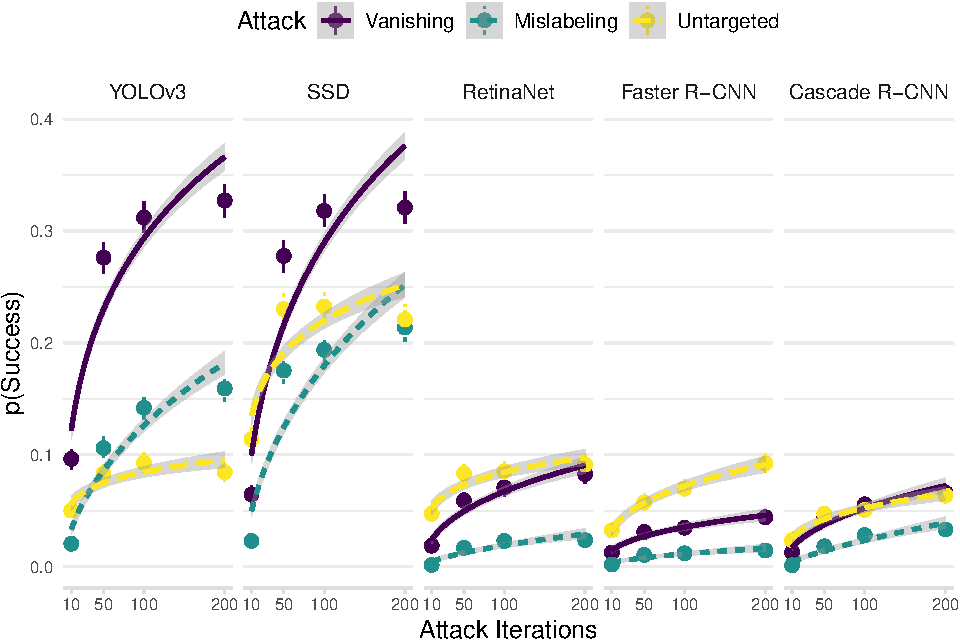
\includegraphics[width=1\linewidth]{imgs/success_trend_graph-1} 

}

\caption{Intent obfuscating attack is feasible for all models and attacks:  We conduct a randomized experiment by resampling COCO images, and within those images randomly sampling correctly predicted target and perturb objects. Then we distort the perturb objects to disrupt the target objects varying the attack iterations. The binned summaries and regression trendlines graph success proportion against attack iterations in the randomized attack experiment. Errors are 95\% confidence intervals and every point aggregates success over 4,000 images. Targeted vanishing and mislabeling attacks obtain significantly greater success on the 1-stage YOLOv3 and SSD than the 2-stage Faster R-CNN and Cascade R-CNN detectors. However, the 1-stage RetinaNet is as resilient as the 2-stage detectors. Moreover, success rates significantly increase with larger attack iterations. Significance is determined at $\alpha < 0.05$ using a Wald z-test on the logistic estimates. Full details are given in Section \ref{sec:rand_att}.}\label{fig:success_trend_graph}
\end{figure*}